\documentclass[11pt]{scrartcl} 

\usepackage{vmargin}
\usepackage{color}
\usepackage{amsthm}
\usepackage{amssymb}
\usepackage{amsmath}
\usepackage{amsfonts}
\usepackage{amstext}
\usepackage{amsbsy}
%\usepackage{mathbbol}
\usepackage{graphicx} 
\usepackage{verbatim}
\usepackage{csvsimple} 
\usepackage{tikz}

%  new definitions
\renewcommand{\div}{\bs{\nabla}\! \cdot \!}
\newcommand{\grad}{\bs{\nabla}}
% extra space
\newcommand{\qq}{\quad\quad}
% common reference commands
\newcommand{\eqt}[1]{Eq.~(\ref{#1})}                     % equation
\newcommand{\fig}[1]{Fig.~\ref{#1}}                      % figure
\newcommand{\tbl}[1]{Table~\ref{#1}}                     % table
\newcommand{\sct}[1]{Section~\ref{#1}}                   % section
\newcommand{\app}[1]{Appendix~\ref{#1}}                   % appendix

\newcommand{\bs}[1]{\mathbf{#1}}
\newcommand{\dd}{\mathrm{d}}
\newcommand{\keff}{k_\textit{eff}}

\newcommand{\be}{\begin{equation}}
\newcommand{\ee}{\end{equation}}
\newcommand{\vn}{\vec{n}}
\newcommand{\vel}{\vec{\mathrm{v}}}
\newcommand{\adj}{\Phi^\dagger_0}
\newcommand{\tcr}[1]{\textcolor{red}{#1}}

% ********* Caption Layout ************
\usepackage{ccaption} % allows special formating of the captions
\captionnamefont{\bf\footnotesize\sffamily} % defines the font of the caption name (e.g. Figure: or Table:)
\captiontitlefont{\footnotesize\sffamily} % defines the font of the caption text (same as above, but not bold)
\setlength{\abovecaptionskip}{0mm} %lowers the distance of captions to the figure

\title{Improved Quasi-Static Method in Rattlesnake}
\author{ 
{\normalsize Zachary M. Prince, Jean C. Ragusa} \\ 
{\normalsize Texas A\&M University} \\  
{\normalsize zachmprince@tamu.edu, jean.ragusa@tamu.edu} \\ 
{\normalsize Yaqi Wang} \\ 
{\normalsize Idaho National Laboratory} \\  
{\normalsize yaqi.wang@inl.gov}
}


\begin{document}
%%%%%%%%%%%%%%%%%%%%%%%%%%%%%%%%%%%%%%%%%%%%%%%%
\maketitle
\pagenumbering{arabic}

%%%%%%%%%%%%%%%%%%%%%%%%%%%%%%%%%%%%%%%%%%%%%%%%
%%%%%%%%%%%%%%%%%%%%%%%%%%%%%%%%%%%%%%%%%%%%%%%%
\section{Introduction}
%%%%%%%%%%%%%%%%%%%%%%%%%%%%%%%%%%%%%%%%%%%%%%%%
%%%%%%%%%%%%%%%%%%%%%%%%%%%%%%%%%%%%%%%%%%%%%%%%
\tcr{Go straight to the point: TREAT testing resumption. The first sentence is a bit generic}
In recent years transient modeling of complex reactor geometries has become a desired prelude to testing.  However, transient modeling has always been especially computationally expensive. Even with the vast improvements in computing technology, current methods have been unbearably slow in real-world cases when retaining sufficient accuracy.  Therefore, methods that improve on computational speed significantly at minimal detriment to accuracy is highly desired.  In particular, the anticipated revitalization \tcr{resumption} of Transient Reactor Testing (TREAT) Facility at Idaho National laboratory (INL) has brought significant attention and opportunity to transient modeling.  TREAT, which was operational from 1954 to 1994, was designed to test fuels by subjecting them to various degrees of neutron pulses, from minor transients to accident cases.  The Department of Energy (DOE) and INL have put substantial effort to developing the modeling architecture for TREAT.  This project addresses the enhancement of transient modeling in TREAT with an improved quasi-static (IQS) method.
\\ \\
The improved quasi-static (IQS) method is a transient spatial kinetics method that involves factorizing flux into space- and time-dependent components.  These components include the flux amplitude and its shape. Amplitude is only time-dependent, while the shape is both space- and time-dependent.  However, the impetus of the method is the assumption that the shape is only weakly dependent on time; therefore, the shape may not require computation at every time step, but only on a macro-time steps. As opposed to other forms of 
quasi-static approximations, the IQS method is not an approximation. The shape is updated consistently and
the results may only differ than those one would obtain using a straight-forward temporal discretization int he sense that the time discretization error in the shape may be larger due to the use of a larger time-step size. 
\tcr{need more references on IQS and some on TREAT. they will kill us without references}
\\ \\
Implementing IQS to Rattlesnake in INL's MOOSE framework is an obvious goal for the project.  Rattlesnake has already been developing methods to be used for TREAT and, with careful planning, IQS can easily be added to the framework as an optional method for problems.  The rest of this summary will briefly describe the derivation of IQS, its current application to Rattlesnake, and anticipated results after further short-term applications.

%%%%%%%%%%%%%%%%%%%%%%%%%%%%%%%%%%%%%%%%%%%%%%%%
%%%%%%%%%%%%%%%%%%%%%%%%%%%%%%%%%%%%%%%%%%%%%%%%
\section{Background}
%%%%%%%%%%%%%%%%%%%%%%%%%%%%%%%%%%%%%%%%%%%%%%%%
%%%%%%%%%%%%%%%%%%%%%%%%%%%%%%%%%%%%%%%%%%%%%%%%

\tcr{Personally, I would put all energy group indices as superscript. up to you.\\}

\tcr{why don't you just say: in this Section, we recall the equations for the IQS method, starting
from the standard multigroup diffusion equations written below:\\}
The multi-group diffusion equation with delayed neutron precursors (DNP) is the first application of this IQS method and will be used to briefly describe IQS derivation:
\begin{align}
\frac{1}{v_g} \frac{\partial \phi_g }{\partial t} =& 
\frac{\chi_{p,g}}{\keff} \sum_{g'=1}^G (1-\beta) \nu_{g'} \Sigma_{f,g'} \phi_{g'} 
-  \left( -\div D_g \grad  + \Sigma_{r,g} \right) \phi_g  \nonumber \\
&  + \sum_{g'\neq g}^G\Sigma_{s,g'\to g} \phi_{g'}  + \sum_{i=1}^I\chi_{d,g,i}\lambda_i C_i \ , \quad 1 \le g \le G 
\end{align}
\be
\frac{dC_i}{dt} = \frac{\beta_i}{k_{eff}}\sum_{g=1}^G\nu_{g} \Sigma_{f,g} \phi_{g} - \lambda_i C_i \ , \quad 1 \le i \le I 
\ee
with
\be
\beta = \sum_{i=1}^I \beta_{i} 
\ee
Factorization is the most important step in the derivation of the IQS method, it is the basis of its existence.  
\tcr{hmmm. existence is technical paper. not my cup of tea. Just be a bit drier and just state things. 
The factorization approach leads to a decomposition of the multigroup flux into the product of a time-dependent amplitude and a space-/time-dependent multigroup shape:}
The group-dependent flux in the above equations is factorized into amplitude (p) and shape (φ):
\be
\phi_g(\vec{r},t)=p(t)\varphi_g(\vec{r},t)
\ee
In order to impose uniqueness \tcr{of the factorization, one imposes:}, between amplitude and shape, the following definition is made:
\be
\left(\phi_g^*,\frac{1}{v_g}\varphi_g\right)=constant
\ee
\tcr{wait a minute: you need to explain the paranthesis notation, preferably with both text and an equation:
summation over energy groups and integration over space\\}
After some manipulation, the amplitude and shape can be solved for by two systems of equations.  The amplitude can be obtained by solving the standard point reactor kinetics equations (PRKE):
\be
\frac{dp}{dt}=\left[\frac{\rho-\bar{\beta}}{\Lambda}\right]p+\sum_{i=1}^I\bar{\lambda}_i\xi_i
\ee
\be
\frac{d\xi_i}{dt}=\frac{\bar{\beta}_i}{\Lambda}-\bar{\lambda}_i\xi_i \quad 1 \le i \le I 
\ee
where the functional coefficients are calculated using the shape function as follows:
\be
\frac{\rho}{\Lambda}=\sum_{g=1}^G\frac{ \left(\phi_g^*,\sum_{g'=1}^G\left\{\frac{1}{k_{eff}} \nu \Sigma_{fg'}+\Sigma_{sg',g}\right\}\varphi_{g'} -\left\{ -\div D_g \grad+\Sigma_{ag}+\sum_{g'>g}^G\Sigma_{sg,g'}\right\}\varphi_g\right)}{\left(\phi_g^*,\frac{1}{v_g}\varphi_g\right)}
\ee
\be
\frac{\bar{\beta}}{\Lambda}=\sum_{i=1}^I\frac{\bar{\beta}_i}{\Lambda}=\frac{1}{k_{eff}}\sum_{i=1}^I\sum_{g=1}^G\frac{(\phi_g^*,\beta_i\nu\Sigma_{fg}\varphi_g)}{\left(\phi_g^*,\frac{1}{v_g}\varphi_g\right)}
\ee
\be
\bar{\lambda}_i=\sum_{g=1}^G\frac{(\phi_g^*,\chi_{g,i}\lambda_iC_i)}{(\phi^*,\chi_{g,i}C_i)}
\ee
\tcr{likely missing 1/p in front of the DNP source term. double check}

Finally, the shape equations are solved for the shape. The shape equations are similar to the orignal diffusion equations:
\begin{align}
\frac{1}{v_g}& \frac{\partial \varphi_g }{\partial t} = \sum_{g'=1}^G\left(\frac{1}{k_{eff}}\nu \Sigma_{fg'}(1-\beta)+\Sigma_{sg',g}\right) \varphi_{g'} - \nonumber \\
& \left( -\div D_g \grad  + \Sigma_{ag}  + \sum_{g'>g}^G\Sigma_{sg,g'} + \frac{1}{v_g}\frac{1}{p}\frac{dp}{dt} \right)\varphi_g + \sum_{i=1}^I\chi_{g,i}\lambda_i C_i \quad 1 \le g \le G 
\label{eq:shape}
\end{align}
However, the amplitude and shape equations form a system of coupled equations: the coefficients appearing in the PRKEs depend upon the shape solution while the shape equation has a kernel dependent on amplitude and its derivative.  Because solving for the shape can be expensive, especially in two or three dimensions, it is attractive to make the assumption that the shape is weakly time-dependent so the shape can be computed after a multitude of PRKE calculations which is the root of IQS.  \tcr{This is depicted schematically in \fig{fig:IQS}.}To visualize:
%
\begin{figure}[h]
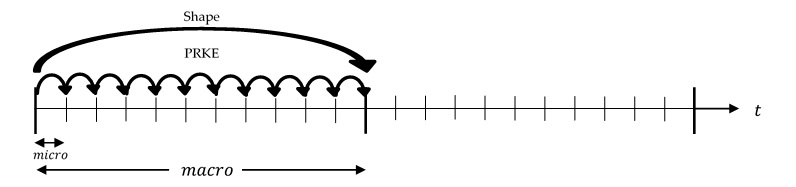
\includegraphics[width=\linewidth]{IQS_visualization.jpg}
\caption{IQS method solution process}
\label{fig:IQS}
\end{figure}
%
\tcr{I am stopping here but you have a good idea now how to modify the rest. thanks!!!!\\}
Additionally, to improve consistency and accuracy, each macro time step can be iterated so the best shape is used to compute power at the micro time steps.  This iteration process must converge the shape such that the uniqueness condition $(\frac{d}{dt}\left(\phi_g^*,\frac{1}{v_g}\varphi_g\right)=0)$ is preserved.

\newpage

%%%%%%%%%%%%%%%%%%%%%%%%%%%%%%%%%%%%%%%%%%%%%%%%
%%%%%%%%%%%%%%%%%%%%%%%%%%%%%%%%%%%%%%%%%%%%%%%%
\section{Implementation into Rattlesnake}
%%%%%%%%%%%%%%%%%%%%%%%%%%%%%%%%%%%%%%%%%%%%%%%%
%%%%%%%%%%%%%%%%%%%%%%%%%%%%%%%%%%%%%%%%%%%%%%%%

MOOSE, or Multiphysics Object-Oriented Simulation Environment, finite-element framework developed by INL equipped with advanced nonlinear solvers.  Rattlesnake is a module of MOOSE meant for neutronics and radiation transport problems.  Rattlesnake is already equipped to solve transient transport and diffusion fully implicitly, but for real problems, these methods are inadequately slow.  IQS is meant to enhance this transient feature.  Rattlesnake utilizes an action system which initiates kernels, user objects, and postprocessors; these would otherwise need to be added to the input file, which would be incredibly overbearing in multi-group problems.  IQS, so far, has been applied to CFEM Diffusion, so this action will be discussed in detail.  The visualized the CFEM Diffusion action: 

\begin{figure}[h]
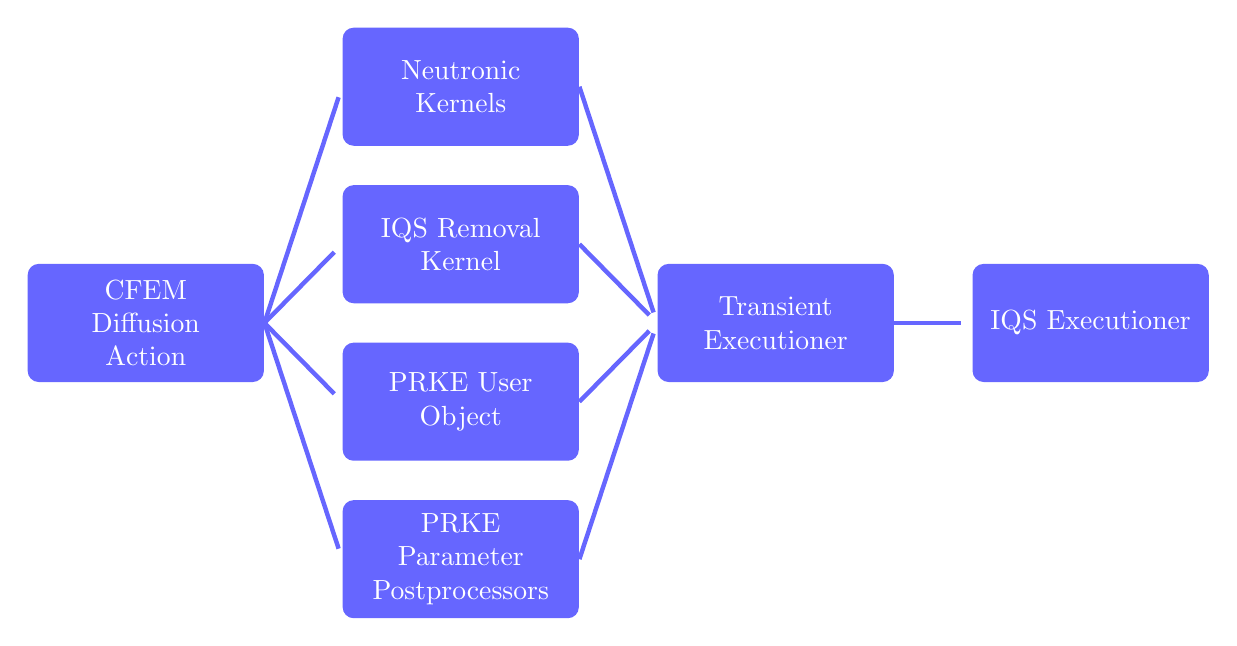
\begin{tikzpicture}[every node/.style = {shape          = rectangle, rounded corners, fill = blue!60, minimum width  = 3cm, minimum height = 1.5cm, align= center, text = white},blue edge/.style  = { -, ultra thick, blue!60, shorten >= 4pt}]
\node(0;0) at (0,0) {CFEM \\ Diffusion \\ Action};
  \node(1;3)  at (4, 3) {Neutronic \\ Kernels};   
  \node(1;1)  at (4, 1) {IQS Removal \\ Kernel}; 
  \node(1;-1)  at (4,-1) {PRKE User \\ Object}; 
  \node(1;-3) at (4,-3) {PRKE \\ Parameter \\ Postprocessors}; 
     \node(2;0)  at (8,0) {Transient \\ Executioner};
     	\node(3;0)  at (12,0) {IQS Executioner};
\foreach \j in {-3,-1,1,3}
  { \draw[blue edge] (0;0.east) -- (1;\j.west); }
\foreach \j in {-3,-1,1,3}
  { \draw[blue edge] (1;\j.east) -- (2;0.west);} 
\draw[blue edge] (2;0.east) -- (3;0.west);         
\end{tikzpicture}
\caption{CFEM Diffusion Action Process Diagram}   
\label{Action}
\end{figure}

%%%%%%%%%%%%%%%%%%%%%%%%%%%%%%%%%%%%%%%%%%%%%%%%
\subsection{Action System}
%%%%%%%%%%%%%%%%%%%%%%%%%%%%%%%%%%%%%%%%%%%%%%%%

IQS defines its uniqueness from its executioner type; however, some changes needed to be made in the Yak action system in order to support IQS execution.   First, changes needed to be made in order to evaluate the shape equation.  The shape equation, after some manipulation, is very similar to the time-dependent flux, as seen in equation (\ref{eq:shape}) which Yak is already set up to solve.  To enable Yak to solve this equation, another kernel was created that evaluated $\frac{1}{vp}\frac{dp}{dt}\varphi$ and added when the IQS executioner is called.  Second, four postprocessors were created in order to calculate the PRKE parameters.  The parameter calculations were separated by $\frac{\bar{\beta}_i}{\Lambda}$ numerator, $\bar{\lambda}_i$ numerator/denominator, $\frac{\rho}{\Lambda}/\frac{\bar{\beta}}{\Lambda}$ denominator, and $\frac{\rho-\bar{\beta}}{\Lambda}$ numerator.  The first three are relatively simple, only relying on material properties and solution quantities.  The $\frac{\rho-\bar{\beta}}{\Lambda}$ numerator requires the use of the Moose save in feature, which saves the residual from a calculated kernel or boundary contribution in the shape evaluation to an auxiliary variable.  Finally, a user object was created to pull together all the postprocessor values and carryout the numerator/denominator divisions that were then passed to the executioner.

%%%%%%%%%%%%%%%%%%%%%%%%%%%%%%%%%%%%%%%%%%%%%%%%
\subsection{Executioner}
%%%%%%%%%%%%%%%%%%%%%%%%%%%%%%%%%%%%%%%%%%%%%%%%

The IQS executioner derives from the Transient executioner in Moose.  The IQS executioner contains a loop over micro time steps that computes the PRKE and then passes p and dp/dt for the Transient executioner to evaluate the shape equation at each macro step.  The PRKE is computed with backward Euler to retain simplicity and insure convergence, but higher order methods are an obvious next step for this computation.   The IQS executioner also supplements Transient’s Picard iteration process by adding its own error criteria: 
\be
Error_{IQS}=\left|\frac{\left(\phi^*_g,\frac{1}{v_g}\varphi_g^n\right)}{\left(\phi_g^*,\frac{1}{v_g}\varphi_g^0\right)}-1\right|
\ee

%%%%%%%%%%%%%%%%%%%%%%%%%%%%%%%%%%%%%%%%%%%%%%%%
%%%%%%%%%%%%%%%%%%%%%%%%%%%%%%%%%%%%%%%%%%%%%%%%
\section{Preliminary Results}
%%%%%%%%%%%%%%%%%%%%%%%%%%%%%%%%%%%%%%%%%%%%%%%%
%%%%%%%%%%%%%%%%%%%%%%%%%%%%%%%%%%%%%%%%%%%%%%%%

This section describes results of an excellent example that tests the IQS implementation and portrays its effectiveness on speed and accuracy.  The example is very simple and computes quickly, it entails a one dimensional, single group, diffusion problem of a heterogeneous slab with a varying absorption cross section.
\\ \\
Figure \ref{fig:power} shows the power at each macro time step, power is defined as the elemental integral of the flux.
\begin{figure}[h]
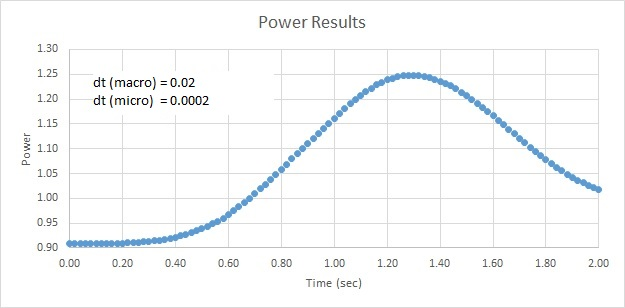
\includegraphics[width=\linewidth]{power_results.jpg}
\caption{Power Results through Flux Integral Postprocessing}
\label{fig:power}
\end{figure}

%%%%%%%%%%%%%%%%%%%%%%%%%%%%%%%%%%%%%%%%%%%%%%%%
%%%%%%%%%%%%%%%%%%%%%%%%%%%%%%%%%%%%%%%%%%%%%%%%
\section{Ongoing Work \& Conclusions}
%%%%%%%%%%%%%%%%%%%%%%%%%%%%%%%%%%%%%%%%%%%%%%%%
%%%%%%%%%%%%%%%%%%%%%%%%%%%%%%%%%%%%%%%%%%%%%%%%

There is much more opportunity to increase the application of IQS.  In the immediate future, IQS will be applied to both DFEM diffusion and $S_n$ transport in Rattlesnake.  Applying IQS to these techniques will be much simpler than the initial implementation to CFEM diffusion because the foundation of the method has already been implemented and only small manipulations of Rattlesnake will be needed.  After this implementation, a multi-dimensional, multi-group test will be created to show how IQS can handle increased complexity and get closer to real-world application.
\\
The derivation and application of IQS has demonstrated to be simple and elegant.  Its implementation into Rattlesnake has proven to be a great fit and its usage for industrial application is inevitable.  The future of this application of IQS is incredibly exciting.  It has the opportunity to greatly enhance the ability to solve complex reactor problems in transient.














\end{document}